\section{Customize}
%The customize window and widgets (spinner/colorpicker)
%\textit{Introduktion til customize fragmentet.\\
%Beskrivelse af arkitekturen i fragmentet\\
%Beskrivelse (med eksempler) af implementationen af de forskellige elementer (knapper osv.) i customize fragmentet}
The customize fragment is the heart of the application, this is where everything is generated and configured.
The fragment can both create new and modify already existing timers, this is the key functionality of the customize fragment.\\
\\
The timers that the guardians already use at the institutions comes in many different colors and timespans.
Therefor is it possible to modify the look, time, and color of the individual timers in the customize fragment.
Furthermore did the guardians state that a good feature would be if either pictograms or other timers were attachable to the timers.\\
\\
Combined with the general idea of the application with a child and timer overview, is the requirements of the features in the customize fragment as follows:\\

\begin{itemize}
	\item Change style of the timer
	\item Change the timespan of the timer
	\item Change the color of the timer and background
	\item Change the color of the timer to be changing gradiently
	\item Attach a pictogram or a timer to the timer
	\item Change the done picture of the timer
	\item Save the timer
	\item Start the timer
\end{itemize}

\color[rgb]{1,0,0} Det hører næsten mere til et design afsnit \color[rgb]{0,0,0}

\subsection{Architecture of Customize}
The customize fragment consists of four main elements, the first element is the style picker where the user can change the style of the timer.
The second element is the time wheels where the user can change the timespan of the timer.
The third is the color pickers where the user can change the colors of the time left, the frame, and the background of the timer.
The last element is the advanced element where the modifications like attachment can be found.
Figure \ref{fig:customize:layout} show how the fragment has been outlined.

\begin{figure}[H]
	\centering
		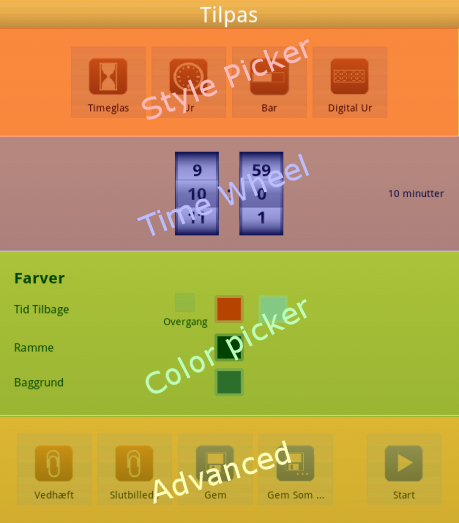
\includegraphics[width=\textwidth]{Images/Implementation/customize_layout.png}
	\caption{An outline of the elements of the customize fragment.}
	\label{fig:customize:layout}
\end{figure}

In the actual customize class has all buttons been initialized as global objects for quick reference.
Since everyone on the WOMBAT project were new to Android programming when the structure of the class were stablished, is all functionality of the items in the customize fragment in this class.
For further development would a refactoring of the entire class be adviced such that all buttons in WOMBAT is handled like the WDialog.\\
To be able to get an overview of the items in the customize fragment has all items been assigned a method which initializes the item e.g. the style chooser in figure \ref{code:customize:style_choser}.
These methods are then referenced from the onCreate method in figure \ref{code:customize:oncreate}.

\begin{figure}[H]
\begin{lstlisting}
private void initStyleChoser() {
	hourglassButton = (Button) getActivity().findViewById(
			R.id.houglassButton);
	hourglassButton.setOnClickListener(new OnClickListener() {

		public void onClick(View v) {
			selectStyle(formFactor.Hourglass);
		}
	});

	timetimerButton = (Button) getActivity().findViewById(
			R.id.timetimerButton);
	timetimerButton.setOnClickListener(new OnClickListener() {

		public void onClick(View v) {
			selectStyle(formFactor.TimeTimer);
		}
	});

	progressbarButton = (Button) getActivity().findViewById(
			R.id.progressbarButton);
	progressbarButton.setOnClickListener(new OnClickListener() {

		public void onClick(View v) {
			selectStyle(formFactor.ProgressBar);
		}
	});

	digitalButton = (Button) getActivity().findViewById(R.id.digitalButton);
	digitalButton.setOnClickListener(new OnClickListener() {

		public void onClick(View v) {
			selectStyle(formFactor.DigitalClock);
		}
	});
}
\end{lstlisting}
\caption{The style choser initialization method, which utilizes the selectStyle that changes the style of the timer and highlights the button.}%
\label{code:customize:style_choser}%
\end{figure}

\begin{figure}[H]
\begin{lstlisting}
public void onActivityCreated(Bundle savedInstanceState) {
	super.onActivityCreated(savedInstanceState);
	currSubP = new SubProfile("", "", 0xff3D3D3D, 0xffFF0000, 0xffB8B8B8,
			0xff000000, 600, false);
	currSubP.save = false;
	currSubP.saveAs = false;

	/********* TIME CHOSER *********/
	initStyleChoser();

	/********* TIMEPICKER *********/
	initTimePicker();

	/********* COLORPICKER *********/
	initColorButtons();

	/********* ATTACHMENT PICKER *********/
	initAttachmentButton();

	/******** BOTTOM MENU ***********/
	initBottomMenu();
}
\end{lstlisting}
\caption{The onCreate method, which calls the button initializers in the same order as they are shown in the layout.}%
\label{code:customize:oncreate}%
\end{figure}

For successors on the WOMBAT project does Eclipse have a keyboard shortcut (F3) which jumps to the method your cursor is at, that can be used to quickly find e.g. the color buttons in the customize class.

\subsection{Buttons in Customize}
There is roughly four kinds of buttons in the customize fragment:

\begin{itemize}
	\item Start, Save, and style buttons
	\item Time picker wheels
	\item Color picker
	\item Attachment and Done picture button
\end{itemize}

\subsubsection*{Start Button}
The style, save, start, and attachment buttons are ordinary Android buttons with a picture attached to the top side.
The differences of these buttons is the onclick event handler which is slightly different from button to button, figure \ref{code:customize:start_button} is the source code of the start button.

\begin{figure}[H]
\begin{lstlisting}
private void initStartButton() {
 startButton = (Button) getActivity().findViewById(
		 R.id.customize_start_button);
 Drawable d;
 if (currSubP.saveAs) {
	 d = getResources().getDrawable(R.drawable.thumbnail_start);
	 startButton.setOnClickListener(new OnClickListener() {

		 public void onClick(View v) {
			 currSubP.addLastUsed(preSubP);
			 guard.saveGuardian(currSubP);
			 currSubP.select();
			 Intent i = new Intent(
					 getActivity().getApplicationContext(),
					 DrawLibActivity.class);
			 startActivity(i);
		 }
	 });
 } else {
				...
		 }
	 });
 }

 startButton
 .setCompoundDrawablesWithIntrinsicBounds(null, d, null, null);
}
\end{lstlisting}
\caption{The source code of the start button, which sets the top image of the button to the drawable \tt thumbnail\_start\_gray}%
\label{code:customize:start_button}%
\end{figure}

\subsubsection*{Time Picker Wheels}
The time picker wheels is a wheel widget created by \url{yuri.kanivets@gmail.com} \cite{web:android:customize:wheel}, these wheels can be customized to mimic the time pickers from the iPhone.
All functionality of the wheel widget is handled by the widget itself and only requires the widget to be imported to Eclipse and added as a library, which is a built in feature in the Android development environment.
To avoid a situation where the user would try to set the time to more than 60 minutes, did we implement a functionality which sets the seconds wheel to zero whenever the minutes wheel is set to 60, this can be seen in figure \ref{code:customize:time_picker_wheels}.

\begin{figure}[H]
\begin{lstlisting}
private int previousMins;
private int previousSecs;
private void initTimePicker() {
	/* Create minute Wheel */
	mins = (WheelView) getActivity().findViewById(R.id.minPicker);
	mins.setViewAdapter(new NumericWheelAdapter(getActivity()
			.getApplicationContext(), 0, 60));
	mins.setCyclic(true);

	/* Add on change listeners for both wheels */
	mins.addChangingListener(new OnWheelChangedListener() {
		public void onChanged(WheelView wheel, int oldValue, int newValue) {
			updateTime(mins.getCurrentItem(), secs.getCurrentItem());

			if (mins.getCurrentItem() == 60) {
				previousMins = 60;
				previousSecs = secs.getCurrentItem();

				secs.setCurrentItem(0);
				secs.setViewAdapter(new NumericWheelAdapter(getActivity()
						.getApplicationContext(), 0, 0));
				secs.setCyclic(false);
			} else if (previousMins == 60) {
				secs.setViewAdapter(new NumericWheelAdapter(getActivity()
						.getApplicationContext(), 0, 60));

				secs.setCurrentItem(previousSecs);
				secs.setCyclic(true);
				previousMins = 0;
			}
		}
	});
}
\end{lstlisting}
\caption{The time picker wheels, with the functionality which ensures the time is never set to more than 60 minutes}%
\label{code:customize:time_picker_wheels}%
\end{figure}


\subsubsection*{Color Picker}
Just like the time picker wheels did we utilize the widget functionality in Android to implement a widget called AmbilWarna (means Take Color in Indonesian), created by Yuku Sugianto \cite{web:android:customize:color}, to handle the color picker.
The color picker widget is a custom dialog which returns the color picked by the user in the widget, the implementation of the color picker widget can be found in figure \ref{code:customize:color_picker}.
\begin{figure}[H]
\begin{lstlisting}
colorGradientButton2 = (Button) getActivity().findViewById(
		R.id.gradientButton_2);
setColor(colorGradientButton2.getBackground(), currSubP.timeSpentColor);
colorGradientButton2.setOnClickListener(new OnClickListener() {
	public void onClick(View v) {
		AmbilWarnaDialog dialog = new AmbilWarnaDialog(getActivity(),
				currSubP.timeSpentColor, new OnAmbilWarnaListener() {
			public void onCancel(AmbilWarnaDialog dialog) {
			}

			public void onOk(AmbilWarnaDialog dialog, int color) {
				currSubP.timeSpentColor = color;
				setColor(colorGradientButton2.getBackground(),
						currSubP.timeSpentColor);
			}
		});
		dialog.show();
	}
});
\end{lstlisting}
\caption{The color picker widget implement on the second "Time Left" button}%
\label{code:customize:color_picker}%
\end{figure}

\subsubsection*{Attachment Button}
The attachment buttons are implemented like the other buttons, but they make use of a custom dialog in WOMBAT.
We created this dialog, because the standard dialogs in Android were very different from the rest of the WOMBAT design.
Also were we unable to define exactly what kind of buttons we wanted in our dialogs.\\
Therefor did we implement the custom dialog which would match the rest of our WOMBAT design and give the ability to control exactly what the buttons on the dialog should look like and what they should do when clicked.
Figure \ref{code:customize:wdialog} is an example of how a dialog could be specified.

\begin{figure}[H]
\begin{lstlisting}
final WDialog attachment1 = new WDialog(getActivity(),
	R.string.attachment_dialog_description);

ModeAdapter adapter = new ModeAdapter(getActivity(),
	android.R.layout.simple_list_item_1, mode);

attachment1.setAdapter(adapter);

attachment1.addButton(R.string.cancel, 1,
	new OnClickListener() {

	public void onClick(View arg0) {
		attachment1.cancel();
	}
});
\end{lstlisting}
\caption{Initialization of the dialog, that appears when the attachment button is clicked, the onItemClickListener is not shown here because of lack of space on the page.}%
\label{code:customize:wdialog}%
\end{figure}